
% Default to the notebook output style

    


% Inherit from the specified cell style.




    
\documentclass{article}

    
    
    \usepackage{graphicx} % Used to insert images
    \usepackage{adjustbox} % Used to constrain images to a maximum size 
    \usepackage{color} % Allow colors to be defined
    \usepackage{enumerate} % Needed for markdown enumerations to work
    \usepackage{geometry} % Used to adjust the document margins
    \usepackage{amsmath} % Equations
    \usepackage{amssymb} % Equations
    \usepackage{eurosym} % defines \euro
    \usepackage[mathletters]{ucs} % Extended unicode (utf-8) support
    \usepackage[utf8x]{inputenc} % Allow utf-8 characters in the tex document
    \usepackage{fancyvrb} % verbatim replacement that allows latex
    \usepackage{grffile} % extends the file name processing of package graphics 
                         % to support a larger range 
    % The hyperref package gives us a pdf with properly built
    % internal navigation ('pdf bookmarks' for the table of contents,
    % internal cross-reference links, web links for URLs, etc.)
    \usepackage{hyperref}
    \usepackage{longtable} % longtable support required by pandoc >1.10
    \usepackage{booktabs}  % table support for pandoc > 1.12.2
    \usepackage{indentfirst}
    \usepackage{amsmath}
    \usepackage{floatrow}
    
    
    \definecolor{orange}{cmyk}{0,0.4,0.8,0.2}
    \definecolor{darkorange}{rgb}{.71,0.21,0.01}
    \definecolor{darkgreen}{rgb}{.12,.54,.11}
    \definecolor{myteal}{rgb}{.26, .44, .56}
    \definecolor{gray}{gray}{0.45}
    \definecolor{lightgray}{gray}{.95}
    \definecolor{mediumgray}{gray}{.8}
    \definecolor{inputbackground}{rgb}{.95, .95, .85}
    \definecolor{outputbackground}{rgb}{.95, .95, .95}
    \definecolor{traceback}{rgb}{1, .95, .95}
    % ansi colors
    \definecolor{red}{rgb}{.6,0,0}
    \definecolor{green}{rgb}{0,.65,0}
    \definecolor{brown}{rgb}{0.6,0.6,0}
    \definecolor{blue}{rgb}{0,.145,.698}
    \definecolor{purple}{rgb}{.698,.145,.698}
    \definecolor{cyan}{rgb}{0,.698,.698}
    \definecolor{lightgray}{gray}{0.5}
    
    % bright ansi colors
    \definecolor{darkgray}{gray}{0.25}
    \definecolor{lightred}{rgb}{1.0,0.39,0.28}
    \definecolor{lightgreen}{rgb}{0.48,0.99,0.0}
    \definecolor{lightblue}{rgb}{0.53,0.81,0.92}
    \definecolor{lightpurple}{rgb}{0.87,0.63,0.87}
    \definecolor{lightcyan}{rgb}{0.5,1.0,0.83}
    
    % commands and environments needed by pandoc snippets
    % extracted from the output of `pandoc -s`
    \providecommand{\tightlist}{%
      \setlength{\itemsep}{0pt}\setlength{\parskip}{0pt}}
    \DefineVerbatimEnvironment{Highlighting}{Verbatim}{commandchars=\\\{\}}
    % Add ',fontsize=\small' for more characters per line
    \newenvironment{Shaded}{}{}
    \newcommand{\KeywordTok}[1]{\textcolor[rgb]{0.00,0.44,0.13}{\textbf{{#1}}}}
    \newcommand{\DataTypeTok}[1]{\textcolor[rgb]{0.56,0.13,0.00}{{#1}}}
    \newcommand{\DecValTok}[1]{\textcolor[rgb]{0.25,0.63,0.44}{{#1}}}
    \newcommand{\BaseNTok}[1]{\textcolor[rgb]{0.25,0.63,0.44}{{#1}}}
    \newcommand{\FloatTok}[1]{\textcolor[rgb]{0.25,0.63,0.44}{{#1}}}
    \newcommand{\CharTok}[1]{\textcolor[rgb]{0.25,0.44,0.63}{{#1}}}
    \newcommand{\StringTok}[1]{\textcolor[rgb]{0.25,0.44,0.63}{{#1}}}
    \newcommand{\CommentTok}[1]{\textcolor[rgb]{0.38,0.63,0.69}{\textit{{#1}}}}
    \newcommand{\OtherTok}[1]{\textcolor[rgb]{0.00,0.44,0.13}{{#1}}}
    \newcommand{\AlertTok}[1]{\textcolor[rgb]{1.00,0.00,0.00}{\textbf{{#1}}}}
    \newcommand{\FunctionTok}[1]{\textcolor[rgb]{0.02,0.16,0.49}{{#1}}}
    \newcommand{\RegionMarkerTok}[1]{{#1}}
    \newcommand{\ErrorTok}[1]{\textcolor[rgb]{1.00,0.00,0.00}{\textbf{{#1}}}}
    \newcommand{\NormalTok}[1]{{#1}}
    
    % Define a nice break command that doesn't care if a line doesn't already
    % exist.
    \def\br{\hspace*{\fill} \\* }
    % Math Jax compatability definitions
    \def\gt{>}
    \def\lt{<}
    % Document parameters
    \title{Homework 7}
    \author{Roly Vicar\'ia \\ STAT501 Fall 2015}    
    
    

    % Pygments definitions
    
\makeatletter
\def\PY@reset{\let\PY@it=\relax \let\PY@bf=\relax%
    \let\PY@ul=\relax \let\PY@tc=\relax%
    \let\PY@bc=\relax \let\PY@ff=\relax}
\def\PY@tok#1{\csname PY@tok@#1\endcsname}
\def\PY@toks#1+{\ifx\relax#1\empty\else%
    \PY@tok{#1}\expandafter\PY@toks\fi}
\def\PY@do#1{\PY@bc{\PY@tc{\PY@ul{%
    \PY@it{\PY@bf{\PY@ff{#1}}}}}}}
\def\PY#1#2{\PY@reset\PY@toks#1+\relax+\PY@do{#2}}

\expandafter\def\csname PY@tok@gd\endcsname{\def\PY@tc##1{\textcolor[rgb]{0.63,0.00,0.00}{##1}}}
\expandafter\def\csname PY@tok@gu\endcsname{\let\PY@bf=\textbf\def\PY@tc##1{\textcolor[rgb]{0.50,0.00,0.50}{##1}}}
\expandafter\def\csname PY@tok@gt\endcsname{\def\PY@tc##1{\textcolor[rgb]{0.00,0.27,0.87}{##1}}}
\expandafter\def\csname PY@tok@gs\endcsname{\let\PY@bf=\textbf}
\expandafter\def\csname PY@tok@gr\endcsname{\def\PY@tc##1{\textcolor[rgb]{1.00,0.00,0.00}{##1}}}
\expandafter\def\csname PY@tok@cm\endcsname{\let\PY@it=\textit\def\PY@tc##1{\textcolor[rgb]{0.25,0.50,0.50}{##1}}}
\expandafter\def\csname PY@tok@vg\endcsname{\def\PY@tc##1{\textcolor[rgb]{0.10,0.09,0.49}{##1}}}
\expandafter\def\csname PY@tok@m\endcsname{\def\PY@tc##1{\textcolor[rgb]{0.40,0.40,0.40}{##1}}}
\expandafter\def\csname PY@tok@mh\endcsname{\def\PY@tc##1{\textcolor[rgb]{0.40,0.40,0.40}{##1}}}
\expandafter\def\csname PY@tok@go\endcsname{\def\PY@tc##1{\textcolor[rgb]{0.53,0.53,0.53}{##1}}}
\expandafter\def\csname PY@tok@ge\endcsname{\let\PY@it=\textit}
\expandafter\def\csname PY@tok@vc\endcsname{\def\PY@tc##1{\textcolor[rgb]{0.10,0.09,0.49}{##1}}}
\expandafter\def\csname PY@tok@il\endcsname{\def\PY@tc##1{\textcolor[rgb]{0.40,0.40,0.40}{##1}}}
\expandafter\def\csname PY@tok@cs\endcsname{\let\PY@it=\textit\def\PY@tc##1{\textcolor[rgb]{0.25,0.50,0.50}{##1}}}
\expandafter\def\csname PY@tok@cp\endcsname{\def\PY@tc##1{\textcolor[rgb]{0.74,0.48,0.00}{##1}}}
\expandafter\def\csname PY@tok@gi\endcsname{\def\PY@tc##1{\textcolor[rgb]{0.00,0.63,0.00}{##1}}}
\expandafter\def\csname PY@tok@gh\endcsname{\let\PY@bf=\textbf\def\PY@tc##1{\textcolor[rgb]{0.00,0.00,0.50}{##1}}}
\expandafter\def\csname PY@tok@ni\endcsname{\let\PY@bf=\textbf\def\PY@tc##1{\textcolor[rgb]{0.60,0.60,0.60}{##1}}}
\expandafter\def\csname PY@tok@nl\endcsname{\def\PY@tc##1{\textcolor[rgb]{0.63,0.63,0.00}{##1}}}
\expandafter\def\csname PY@tok@nn\endcsname{\let\PY@bf=\textbf\def\PY@tc##1{\textcolor[rgb]{0.00,0.00,1.00}{##1}}}
\expandafter\def\csname PY@tok@no\endcsname{\def\PY@tc##1{\textcolor[rgb]{0.53,0.00,0.00}{##1}}}
\expandafter\def\csname PY@tok@na\endcsname{\def\PY@tc##1{\textcolor[rgb]{0.49,0.56,0.16}{##1}}}
\expandafter\def\csname PY@tok@nb\endcsname{\def\PY@tc##1{\textcolor[rgb]{0.00,0.50,0.00}{##1}}}
\expandafter\def\csname PY@tok@nc\endcsname{\let\PY@bf=\textbf\def\PY@tc##1{\textcolor[rgb]{0.00,0.00,1.00}{##1}}}
\expandafter\def\csname PY@tok@nd\endcsname{\def\PY@tc##1{\textcolor[rgb]{0.67,0.13,1.00}{##1}}}
\expandafter\def\csname PY@tok@ne\endcsname{\let\PY@bf=\textbf\def\PY@tc##1{\textcolor[rgb]{0.82,0.25,0.23}{##1}}}
\expandafter\def\csname PY@tok@nf\endcsname{\def\PY@tc##1{\textcolor[rgb]{0.00,0.00,1.00}{##1}}}
\expandafter\def\csname PY@tok@si\endcsname{\let\PY@bf=\textbf\def\PY@tc##1{\textcolor[rgb]{0.73,0.40,0.53}{##1}}}
\expandafter\def\csname PY@tok@s2\endcsname{\def\PY@tc##1{\textcolor[rgb]{0.73,0.13,0.13}{##1}}}
\expandafter\def\csname PY@tok@vi\endcsname{\def\PY@tc##1{\textcolor[rgb]{0.10,0.09,0.49}{##1}}}
\expandafter\def\csname PY@tok@nt\endcsname{\let\PY@bf=\textbf\def\PY@tc##1{\textcolor[rgb]{0.00,0.50,0.00}{##1}}}
\expandafter\def\csname PY@tok@nv\endcsname{\def\PY@tc##1{\textcolor[rgb]{0.10,0.09,0.49}{##1}}}
\expandafter\def\csname PY@tok@s1\endcsname{\def\PY@tc##1{\textcolor[rgb]{0.73,0.13,0.13}{##1}}}
\expandafter\def\csname PY@tok@kd\endcsname{\let\PY@bf=\textbf\def\PY@tc##1{\textcolor[rgb]{0.00,0.50,0.00}{##1}}}
\expandafter\def\csname PY@tok@sh\endcsname{\def\PY@tc##1{\textcolor[rgb]{0.73,0.13,0.13}{##1}}}
\expandafter\def\csname PY@tok@sc\endcsname{\def\PY@tc##1{\textcolor[rgb]{0.73,0.13,0.13}{##1}}}
\expandafter\def\csname PY@tok@sx\endcsname{\def\PY@tc##1{\textcolor[rgb]{0.00,0.50,0.00}{##1}}}
\expandafter\def\csname PY@tok@bp\endcsname{\def\PY@tc##1{\textcolor[rgb]{0.00,0.50,0.00}{##1}}}
\expandafter\def\csname PY@tok@c1\endcsname{\let\PY@it=\textit\def\PY@tc##1{\textcolor[rgb]{0.25,0.50,0.50}{##1}}}
\expandafter\def\csname PY@tok@kc\endcsname{\let\PY@bf=\textbf\def\PY@tc##1{\textcolor[rgb]{0.00,0.50,0.00}{##1}}}
\expandafter\def\csname PY@tok@c\endcsname{\let\PY@it=\textit\def\PY@tc##1{\textcolor[rgb]{0.25,0.50,0.50}{##1}}}
\expandafter\def\csname PY@tok@mf\endcsname{\def\PY@tc##1{\textcolor[rgb]{0.40,0.40,0.40}{##1}}}
\expandafter\def\csname PY@tok@err\endcsname{\def\PY@bc##1{\setlength{\fboxsep}{0pt}\fcolorbox[rgb]{1.00,0.00,0.00}{1,1,1}{\strut ##1}}}
\expandafter\def\csname PY@tok@mb\endcsname{\def\PY@tc##1{\textcolor[rgb]{0.40,0.40,0.40}{##1}}}
\expandafter\def\csname PY@tok@ss\endcsname{\def\PY@tc##1{\textcolor[rgb]{0.10,0.09,0.49}{##1}}}
\expandafter\def\csname PY@tok@sr\endcsname{\def\PY@tc##1{\textcolor[rgb]{0.73,0.40,0.53}{##1}}}
\expandafter\def\csname PY@tok@mo\endcsname{\def\PY@tc##1{\textcolor[rgb]{0.40,0.40,0.40}{##1}}}
\expandafter\def\csname PY@tok@kn\endcsname{\let\PY@bf=\textbf\def\PY@tc##1{\textcolor[rgb]{0.00,0.50,0.00}{##1}}}
\expandafter\def\csname PY@tok@mi\endcsname{\def\PY@tc##1{\textcolor[rgb]{0.40,0.40,0.40}{##1}}}
\expandafter\def\csname PY@tok@gp\endcsname{\let\PY@bf=\textbf\def\PY@tc##1{\textcolor[rgb]{0.00,0.00,0.50}{##1}}}
\expandafter\def\csname PY@tok@o\endcsname{\def\PY@tc##1{\textcolor[rgb]{0.40,0.40,0.40}{##1}}}
\expandafter\def\csname PY@tok@kr\endcsname{\let\PY@bf=\textbf\def\PY@tc##1{\textcolor[rgb]{0.00,0.50,0.00}{##1}}}
\expandafter\def\csname PY@tok@s\endcsname{\def\PY@tc##1{\textcolor[rgb]{0.73,0.13,0.13}{##1}}}
\expandafter\def\csname PY@tok@kp\endcsname{\def\PY@tc##1{\textcolor[rgb]{0.00,0.50,0.00}{##1}}}
\expandafter\def\csname PY@tok@w\endcsname{\def\PY@tc##1{\textcolor[rgb]{0.73,0.73,0.73}{##1}}}
\expandafter\def\csname PY@tok@kt\endcsname{\def\PY@tc##1{\textcolor[rgb]{0.69,0.00,0.25}{##1}}}
\expandafter\def\csname PY@tok@ow\endcsname{\let\PY@bf=\textbf\def\PY@tc##1{\textcolor[rgb]{0.67,0.13,1.00}{##1}}}
\expandafter\def\csname PY@tok@sb\endcsname{\def\PY@tc##1{\textcolor[rgb]{0.73,0.13,0.13}{##1}}}
\expandafter\def\csname PY@tok@k\endcsname{\let\PY@bf=\textbf\def\PY@tc##1{\textcolor[rgb]{0.00,0.50,0.00}{##1}}}
\expandafter\def\csname PY@tok@se\endcsname{\let\PY@bf=\textbf\def\PY@tc##1{\textcolor[rgb]{0.73,0.40,0.13}{##1}}}
\expandafter\def\csname PY@tok@sd\endcsname{\let\PY@it=\textit\def\PY@tc##1{\textcolor[rgb]{0.73,0.13,0.13}{##1}}}

\def\PYZbs{\char`\\}
\def\PYZus{\char`\_}
\def\PYZob{\char`\{}
\def\PYZcb{\char`\}}
\def\PYZca{\char`\^}
\def\PYZam{\char`\&}
\def\PYZlt{\char`\<}
\def\PYZgt{\char`\>}
\def\PYZsh{\char`\#}
\def\PYZpc{\char`\%}
\def\PYZdl{\char`\$}
\def\PYZhy{\char`\-}
\def\PYZsq{\char`\'}
\def\PYZdq{\char`\"}
\def\PYZti{\char`\~}
% for compatibility with earlier versions
\def\PYZat{@}
\def\PYZlb{[}
\def\PYZrb{]}
\makeatother


    % Exact colors from NB
    \definecolor{incolor}{rgb}{0.0, 0.0, 0.5}
    \definecolor{outcolor}{rgb}{0.545, 0.0, 0.0}



    
    % Prevent overflowing lines due to hard-to-break entities
    \sloppy 
    % Setup hyperref package
    \hypersetup{
      breaklinks=true,  % so long urls are correctly broken across lines
      colorlinks=true,
      urlcolor=blue,
      linkcolor=darkorange,
      citecolor=darkgreen,
      }
    % Slightly bigger margins than the latex defaults
    
    \geometry{verbose,tmargin=1in,bmargin=1in,lmargin=1in,rmargin=1in}
    
    

    \begin{document}
    
    
    \maketitle
    
    

    
    \subsubsection{Question 1}\label{question-1}

\begin{enumerate}
\def\labelenumi{\alph{enumi})}
\item
  FALSE. The null hypothesis in the Ryan-Joiner test is that the errors
  are normally distributed. So a small p-value would lead us to reject
  the null hypothesis and conclude they are NOT normally distributed.
\item
  FALSE. The confidence interval for the mean response can be valid even
  when the Normality requirement is not satisfied if there is a
  sufficiently large data set. The prediction interval, however,
  strongly relies on the normality requirement.
\item
  TRUE
\item
  TRUE
\item
  FALSE. We could also code the variable as 0, 1, 2, 3, 4.
\end{enumerate}

    \subsubsection{Question 2}\label{question-2}

\begin{enumerate}
\def\labelenumi{\alph{enumi})}
\tightlist
\item
  \(Mort = 1006.2 - 15.35 Edu + 4.214 Nwt - 2.150 Jant + 1.624 Rain + 18.55 Nox + 0.537 Hum - 0.35 Inc\)
\end{enumerate}

SSE = 60417; df = 48

\begin{enumerate}
\def\labelenumi{\alph{enumi})}
\setcounter{enumi}{1}
\tightlist
\item
  \(F^* = \frac{SSE(Reduced) - SSE(Full)}{df_R - df_F} \div \frac{SSE(Full)}{df_F} = \frac{60948 - 60417}{50-48} \div \frac{60417}{48} = 0.211\)
\end{enumerate}

F distribution with 2 DF in numerator and 48 DF in denominator:
\(P(X > 0.211) = 1 - 0.189479 = 0.81\), therefore, we can conclude that
the variables do not provide significant information about the response.

\begin{enumerate}
\def\labelenumi{\alph{enumi})}
\setcounter{enumi}{2}
\tightlist
\item
  \(Mort = 1028.2 - 15.59 Edu + 4.181 Nwt - 2.131 Jant + 1.633 Rain + 18.41 Nox\)
\end{enumerate}


\begin{figure}[h!]
 \centering
 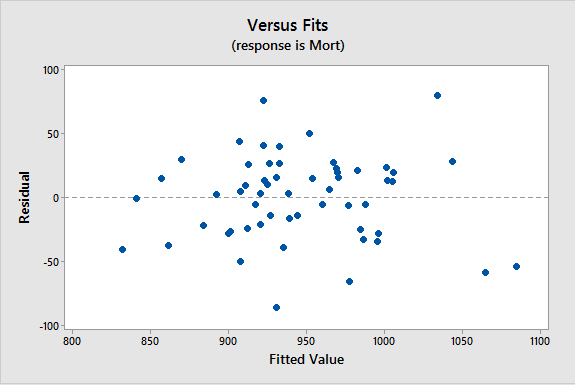
\includegraphics[scale=.5]{./images/scatterplot_residuals-vs-fitted.png}
 % scatterplot_residuals-vs-fitted.png: 575x385 pixel, 96dpi, 15.21x10.19 cm, bb=0 0 431 289
\end{figure}

Scanning the scatterplot
of residuals vs fitted values, it does appear that the vertical average
remains close to 0. This affirms the \textbf{L} condition. Also, the
vertical spread of the residuals remains fairly constant as we scan the
plot from left to right, which affirms the \textbf{E} condition. There
do not appear to be any outliers.

\begin{figure}[h!]
 \centering
 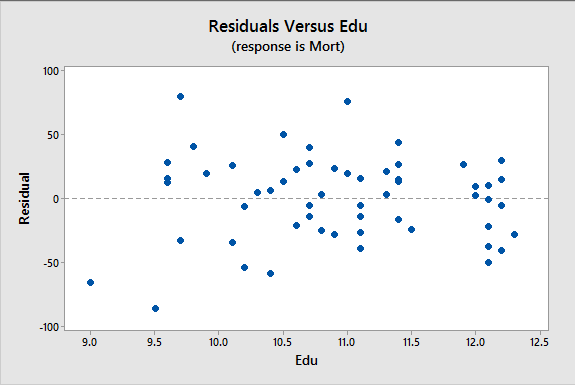
\includegraphics[scale=.5]{./images/scatterplot_residuals-vs-Edu.png}
 % scatterplot_residuals-vs-Edu.png: 575x385 pixel, 96dpi, 15.21x10.19 cm, bb=0 0 431 289
\end{figure}

Looking at the scatterplot of residuals vs Edu, it appears that the vertical average of
the residuals remains approximately 0 (affirming the \textbf{L}
condition), and that the vertical spread of the residuals is fairly
constant (affirming the \textbf{E} condition).

\begin{figure}[h!]
 \centering
 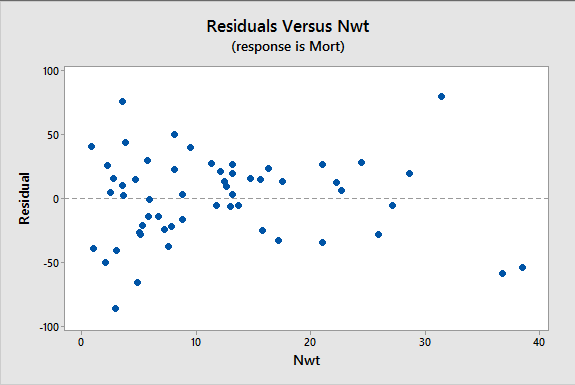
\includegraphics[scale=.5]{./images/scatterplot_residuals-vs-Nwt.png}
 % scatterplot_residuals-vs-Nwt.png: 575x385 pixel, 96dpi, 15.21x10.19 cm, bb=0 0 431 289
\end{figure}

The scatterplot of residuals vs Nwt seems to affirm the \textbf{L}
condition since the vertical average of the residuals appears close to
0, but the vertical spread of the residuals does not seem constant. The
spread seems largest for smaller values of Nwt, less than 10.

\begin{figure}[h!]
 \centering
 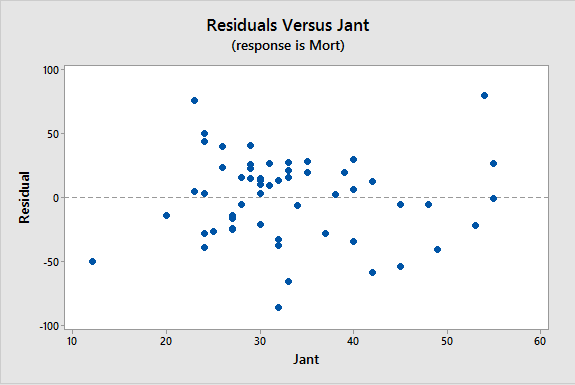
\includegraphics[scale=.5]{./images/scatterplot_residuals-vs-Jant.png}
 % scatterplot_residuals-vs-Jant.png: 575x385 pixel, 96dpi, 15.21x10.19 cm, bb=0 0 431 289
\end{figure}

The scatterplot of residuals vs Jant looks OK. Vertical average of
residuals seems close to 0 and spread seems fairly constant, affirming
both \textbf{L} and \textbf{E} conditions.

\newpage
\begin{figure}[h!]
 \centering
 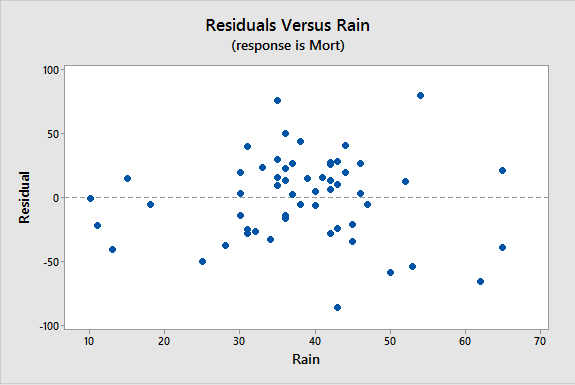
\includegraphics[scale=.5]{./images/scatterplot_residuals-vs-Rain.png}
 % scatterplot_residuals-vs-Rain.png: 575x385 pixel, 96dpi, 15.21x10.19 cm, bb=0 0 431 289
\end{figure}


The residuals vs Rain plot also looks good. Both the \textbf{L} and
\textbf{E} conditions appear satisfied.

\begin{figure}[h!]
 \centering
 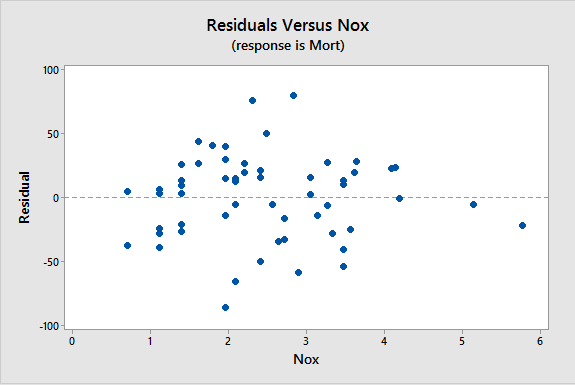
\includegraphics[scale=.5]{./images/scatterplot_residuals-vs-Nox.png}
 % scatterplot_residuals-vs-Nox.png: 575x385 pixel, 96dpi, 15.21x10.19 cm, bb=0 0 431 289
\end{figure}
The residuals vs Nox plot looks OK. Vertical average of residuals seems
close to 0 and the spreads seems fairly constant. A few more spread out
values around Nox = 2, but I don't think it's enough to be suspicious.

\begin{figure}[h!]
 \centering
 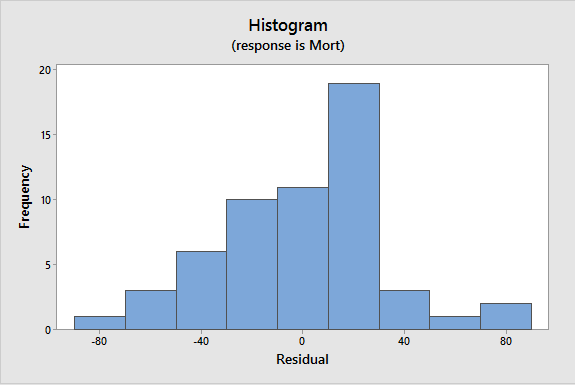
\includegraphics[scale=.5]{./images/histogram_residuals.png}
 % histogram_residuals.png: 575x385 pixel, 96dpi, 15.21x10.19 cm, bb=0 0 431 289
\end{figure}

The histogram doesn't have a perfect
bell shape, and looks slightly skewed, but not enough to confirm
violation of normality.

\newpage
\begin{figure}[h!]
 \centering
 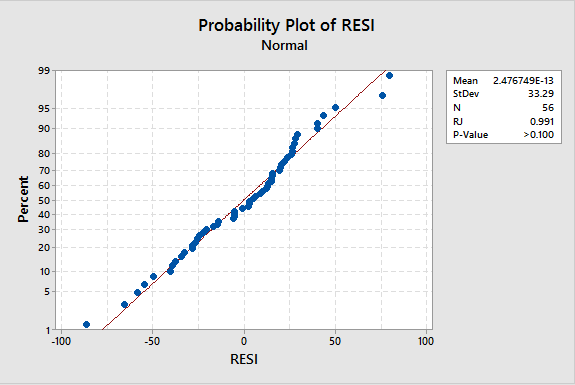
\includegraphics[scale=.5]{./images/probabilityPlot_residuals.png}
 % probabilityPlot_residuals.png: 575x385 pixel, 96dpi, 15.21x10.19 cm, bb=0 0 431 289
\end{figure}

The probability plot and Ryan-Joiner test
support the normality condition of the errors. The test shows a
\emph{p}-value \textgreater{} 0.1 which says we fail to reject the null
hypothesis and conclude that the errors are normally distributed.

\begin{figure}[!h]
  \begin{floatrow}
   \ffigbox{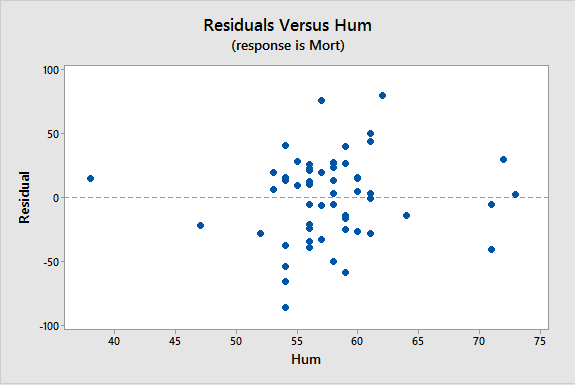
\includegraphics[scale=0.5]{./images/scatterplot_residuals-vs-Hum.png}}{}
   \ffigbox{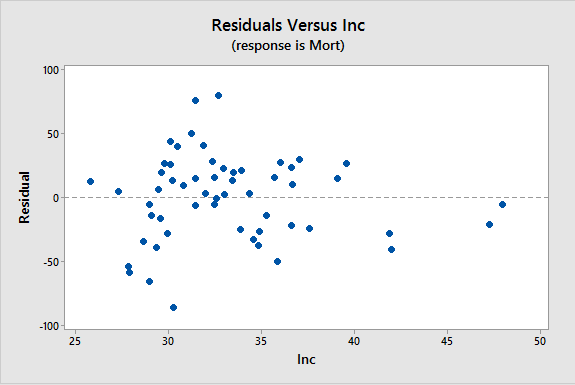
\includegraphics[scale=0.5]{./images/scatterplot_residuals-vs-Inc.png}}{}
  \end{floatrow}
\end{figure}
The scatterplots of residuals vs Hum and Inc seem pretty unremarkable. They
don't show any indication of strong linear or simple nonlinear trends.
They don't appear to warrant being added to the model.

\begin{enumerate}
\def\labelenumi{\alph{enumi})}
\setcounter{enumi}{3}
\item
  The 95\% confidence interval for E(Mort) is (946.273, 978.945). This
  interval can be interpreted as saying that we can be 95\% confident
  that the average mortality rate (age adjusted per 100,000 population)
  for all cities with 10 median years of education, 15 percent non-white
  population, 35 degrees Fahrenheit mean January temperature, 40 inches
  annual rainfall, and 2 units of log(nitrous oxide concentration in
  parts per billion), will be between 946.273 and 978.945.
\item
  The 95\% prediction interval for Mort is (890.605, 1034.61). This
  interval can be interpreted as saying that we can be 95\% confident
  that the mortality rate for a new city with 10 median years of
  education, 15 percent non-white population, 35 degrees Fahrenheit mean
  January temperature, 40 inches annual rainfall, and 2 units of
  log(nitrous oxide concentration in parts per billion), will be between
  890.605 and 1034.61. This interval is wider than the confidence
  interval because it always has an extra MSE term than the confidence
  interval formula.
\end{enumerate}

    \subsubsection{Question 3}\label{question-3}

The \textbf{X} matrix would be a 200 x 5 matrix where each row
corresponds to a record from the data set. The columns are: 1) 1's which
correspond to the \(\beta_0\) constant term, 2) body weight, 3) gender
(0=male,1=female), 4) age, and 5) interaction gender x age.

\newpage
    \subsubsection{Question 4}\label{question-4}

\begin{enumerate}
\def\labelenumi{\alph{enumi})}
\item
  At first glance, it looks like there is an interaction between degree
  and years of experience since it looks like the Masters line is not
  parallel to the other lines. However, upon further observation, I
  believe that the Masters data has an outlier that is a very
  influential point affecting the slope of that line. If we were to
  remove the data point at around 20 years of experience, I suspect that
  the 3 lines would be almost parallel. Which would indicate that there
  is no interaction between degree and years of experience.
\item
  \(Salary = 40.77 + 2.158 YrsExp\)

  \begin{enumerate}
  \def\labelenumii{\roman{enumii})}
  \tightlist
  \item
    SSE = 12412.8
  \item
    61
  \end{enumerate}
\item
  \(Salary = 29.27 + 1.841 YrsExp + 28.36 Deg1 + 10.71 Deg2\)

  \begin{enumerate}
  \def\labelenumii{\roman{enumii})}
  \tightlist
  \item
    SSE = 4948
  \item
    59
  \end{enumerate}
\item
  \(F^* = \frac{SSE(Reduced) - SSE(Full)}{df_R - df_F} \div \frac{SSE(Full)}{df_F} = \frac{12412.8 - 4948}{61 - 59} \div \frac{4948}{59} = 44.505\)
\item
  \begin{enumerate}
  \def\labelenumii{\roman{enumii})}
  \tightlist
  \item
    Df numerator=2, Df denominator=59
  \item
    \emph{p}-value = 0.000 The conclusion we can draw from this is that
    the variables deg1 and deg2 provide significant information about
    the response.
  \end{enumerate}
\item
  \begin{enumerate}
  \def\labelenumii{\roman{enumii})}
  \tightlist
  \item
    \(Salary = 29.27 + 1.841 YrsExp + 28.36 Deg1 + 10.71 Deg2\)
  \item
    \(Salary = 29.27 + 1.841 YrsExp\) (Deg1 = 0, Deg2 = 0)
  \item
    \(Salary = (29.27+10.71) YrsExp\) (Deg1 = 0, Deg2 = 1)
  \item
    \(Salary = (29.27+28.36) YrsExp\) (Deg1 = 1, Deg2 = 0)
  \end{enumerate}
\item
  \begin{enumerate}
  \def\labelenumii{\roman{enumii})}
  \tightlist
  \item
    The coefficient that multiplies the variable Deg1 represents the
    difference in mean salary for employees with PhD's versus employees
    with Bachelor's degrees, assuming the same value for years of
    experience.
  \item
    The coefficient that multiplies the variable Deg2 represents the
    difference in mean salary for employees with Master's degrees versus
    employees with Bachelor's degrees, assuming the same value for the
    years of experience.
  \end{enumerate}
\item
  One way to do it could be to have indicator variables for managers
  with Bachelor's and one indicator variable for managers with Master's
  such that when both are equal to 0 denotes a manager with a PhD. The
  coefficient of interest would then be the coefficient that multiplies
  the variable for Master's degree managers.
\item
  \(Salary = 26.94 + 2.206 YrsExp + 31.26 Deg1 + 13.73 Deg2 - 0.427 YrsExp*Deg1 - 0.471 YrsExp*Deg2\)
\end{enumerate}

\(H_0: \beta_4 = \beta_5 = 0\), \(H_a:\) at least one of \(\beta_4, \beta_5\) is not equal to 0 \\

Test statistic: \(F^* = \frac{SSE(Reduced) - SSE(Full)}{df_R - df_F} \div \frac{SSE(Full)}{df_F} = \frac{4948 - 4867.1}{59 - 57} \div \frac{4867.1}{57} = 0.474\)

This test statistic has a \emph{p}-value of 1 - 0.37506 = 0.625.
Therefore we cannot reject the null hypothesis and conclude that there
is no interaction between highest degree attained and years of
experience.

\newpage
    \subsubsection{Question 5}\label{question-5}

\begin{enumerate}
\def\labelenumi{\alph{enumi})}
\tightlist
\item
  Only (iii) is true. The salary regression lines are:
\begin{align*}
Salary_{male} &= 50 + 20GPA + .07IQ + .01 GPA*IQ \\
Salary_{fem} &= 50 + 20GPA + .07IQ + 35 + .01 GPA*IQ - 10 GPA
\end{align*}
We can see from the equations that female salary is greater as long as
GPA is less than 3.5. After 3.5, then male salaries are greater.
\end{enumerate}

\begin{enumerate}
\def\labelenumi{\alph{enumi})}
\setcounter{enumi}{1}
\item
  137.1
\item
  I agree there is reason to doubt the interaction between GPA and IQ
  since it is such a small value, but we would need to run a
  \emph{t}-test to comment further.
\end{enumerate}


    % Add a bibliography block to the postdoc
    
    
    
    \end{document}
